\chapter{Phase 2: Conformal prediction, OOD, MC Dropout, K-fold CV}
\label{ch:phase2}

% ~15-18 pages

\section{Split conformal prediction}
% - Recap of the algorithm with the binary specialisation.
% - Threshold $\hat q$ fitted on the validation set, evaluated on test.
% - Targets $\alpha = 0.10, 0.05$.

% Table of conformal results per model (binary):
% \input{tables/tab_phase2_conformal_binary}  % You can extend the
% generator to dump this if needed; CSVs are at master/results/phase2/.

% Discuss:
% - Empirical marginal coverage tracks the target (88-93\% for $\alpha=0.10$,
%   95-97\% for $\alpha=0.05$) — confirming the algorithm's validity.
% - APS produces "abstain" sets (\{0,1\}) more often than LAC, which is
%   clinically more useful than empty sets.
% - VGG16 + LAC achieves the highest singleton-correct rate (98.05\%).

\section{Out-of-distribution detection}
% \begin{figure}[t]
%   \centering
%   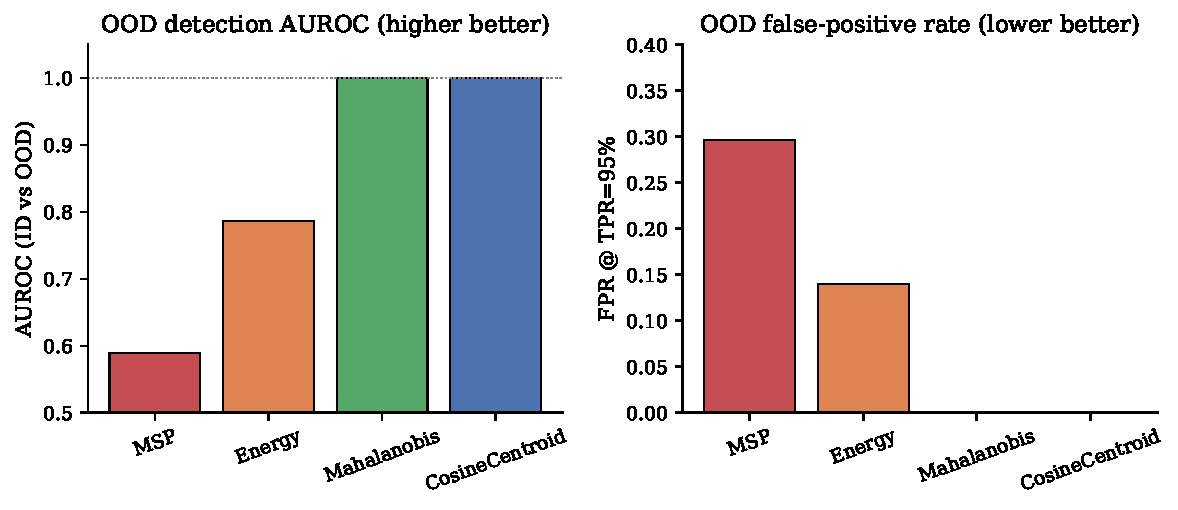
\includegraphics[width=0.95\linewidth]{figures/fig_phase2_ood.pdf}
%   \caption{OOD detection: AUROC (left) and FPR @ TPR=95\% (right) for
%   four scoring methods. ID is the APTOS test set; OOD is 300 synthetic
%   uniform-noise images preprocessed for DenseNet121.}
%   \label{fig:phase2-ood}
% \end{figure}
%
% - MSP fails (AUROC 0.59) — softmax over-confidence on noise.
% - Energy is decent (AUROC 0.79).
% - Mahalanobis and cosine-centroid achieve perfect AUROC 1.0 — feature-
%   space distances easily separate noise from real fundus images.
% - Caveat: noise is the easy case. Real cross-dataset OOD evaluation
%   (e.g.\ on chest X-ray inputs or Messidor-2 with different camera) is
%   more meaningful future work.

\section{Monte Carlo Dropout}
% - Two dropout-equipped variants: cnn\_mcd and resnet50\_mcd.
% - $T = 30$ stochastic forward passes at inference.
% - resnet50\_mcd is the strongest single model (96.18\% test acc),
%   beating the non-dropout ResNet50 (95.27\%).
% - $\sigma$ across MC samples is 3-4$\times$ higher on incorrect
%   predictions — the uncertainty signal is informative.

\section{K-fold cross-validation on ResNet50}
% Auto-generated by master/generate_thesis_tables.py
% Do not edit by hand — re-run the generator instead.
\begin{table}[t]
  \centering
  \caption{ResNet50 5-fold cross-validation results. The held-out test set ($N = 550$) is fixed across folds; only the train/val split varies. Mean test accuracy: $95.64 \pm 0.18$\%.}
  \label{tab:phase2-kfold}
  \small
  \begin{tabular}{ccccccc}
    \toprule
    Fold & Epochs & Best val (\%) & Test acc (\%) & Test AUC & Time (min) \\
    \midrule
    1 & 8 & 95.99 & 95.82 & 0.9867 & 8.5 \\
2 & 21 & 97.11 & 95.82 & 0.9882 & 25.0 \\
3 & 22 & 98.07 & 95.45 & 0.9898 & 38.8 \\
4 & 15 & 97.75 & 95.64 & 0.9903 & 16.5 \\
5 & 25 & 97.59 & 95.45 & 0.9900 & 30.0 \\
    \bottomrule
  \end{tabular}
\end{table}

% \begin{figure}[t]
%   \centering
%   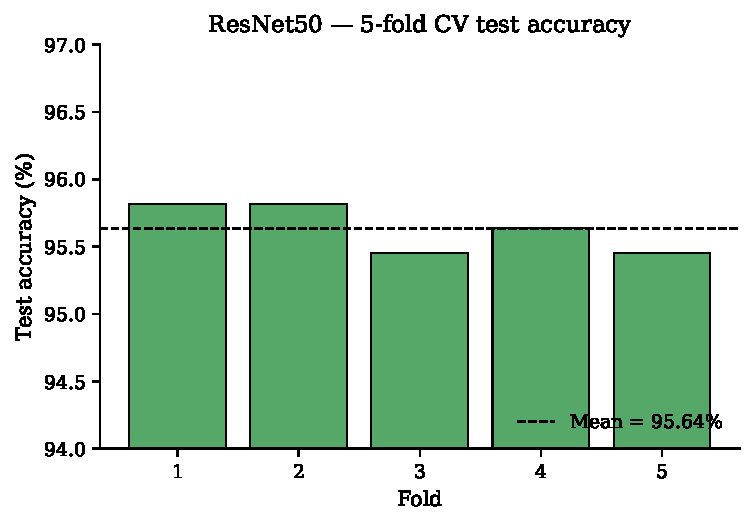
\includegraphics[width=0.65\linewidth]{figures/fig_phase2_kfold.pdf}
%   \caption{ResNet50 5-fold cross-validation test accuracy. Mean and
%   $\pm$1\,$\sigma$ shown; the fixed test set is identical across folds.}
%   \label{fig:phase2-kfold}
% \end{figure}
%
% - Test acc $95.64 \pm 0.18$\,\%, AUC $0.989 \pm 0.002$.
% - Tight standard deviation — the single-split estimate from Phase 1 was
%   representative, not lucky.
% - Combined with the Phase 1 ensemble's 96.55\%, the gap is ~5$\sigma$,
%   confirming that ensembling helps.

\section{Streamlit application integration}
% - The trained models, conformal thresholds and uncertainty signals are
%   exposed in the Streamlit app via two new tabs:
%   * "Predict" gains an "Show uncertainty" checkbox surfacing the
%     ensemble mean, std, predictive entropy and a refer-to-clinician
%     decision.
%   * A new "5-stage grading" tab uses the multi-class models from Phase 3
%     (\cref{ch:phase3}) and shows the conformal prediction set
%     graphically.
% - The app runs entirely on a CPU laptop; no GPU required.

\section{Lessons from Phase 2}
% - Conformal prediction is "free" — no retraining, only a calibration set.
%   It transforms an uncalibrated point predictor into a statistically
%   valid set predictor.
% - MC Dropout is the cheapest Bayesian approximation; it requires
%   retraining with dropout layers but no architectural overhaul.
% - K-fold CV is computationally expensive (5 ResNet50 trainings ≈ 2
%   hours on CPU) but pins down the variance estimate.
% - OOD evaluation against synthetic noise is too easy. Real cross-
%   dataset OOD is required for a thorough study.
